%%%%%%%%%%%%%%%%%%%%%%%%%%%%%%%%%%%%%%%%%
% Beamer Presentation
% LaTeX Template
% Version 1.0 (10/11/12)
%
% This template has been downloaded from:
% http://www.LaTeXTemplates.com
%
% License:
% CC BY-NC-SA 3.0 (http://creativecommons.org/licenses/by-nc-sa/3.0/)
%
%%%%%%%%%%%%%%%%%%%%%%%%%%%%%%%%%%%%%%%%%

%----------------------------------------------------------------------------------------
%	PACKAGES AND THEMES
%----------------------------------------------------------------------------------------

\documentclass[utf8]{beamer}

\RequirePackage[croatian]{babel}

\usepackage{datetime}
\usepackage{adjustbox}
\usepackage{float}

\usepackage{listings}
\usepackage{xcolor}

\colorlet{punct}{red!60!black}
\definecolor{background}{HTML}{EEEEEE}
\definecolor{delim}{RGB}{20,105,176}
\colorlet{numb}{magenta!60!black}

\lstdefinelanguage{json}{
    basicstyle=\tiny\ttfamily,
    stepnumber=1,
    numbersep=8pt,
    showstringspaces=false,
    breaklines=true,
    backgroundcolor=\color{background},
    literate=
     *{0}{{{\color{numb}0}}}{1}
      {1}{{{\color{numb}1}}}{1}
      {2}{{{\color{numb}2}}}{1}
      {3}{{{\color{numb}3}}}{1}
      {4}{{{\color{numb}4}}}{1}
      {5}{{{\color{numb}5}}}{1}
      {6}{{{\color{numb}6}}}{1}
      {7}{{{\color{numb}7}}}{1}
      {8}{{{\color{numb}8}}}{1}
      {9}{{{\color{numb}9}}}{1}
      {:}{{{\color{punct}{:}}}}{1}
      {,}{{{\color{punct}{,}}}}{1}
      {\{}{{{\color{delim}{\{}}}}{1}
      {\}}{{{\color{delim}{\}}}}}{1}
      {[}{{{\color{delim}{[}}}}{1}
      {]}{{{\color{delim}{]}}}}{1},
}

\lstset{language=Python, tabsize=4}

% naredba \engl
\newcommand{\engl}[1]{(engl.~\emph{#1})}

% naredbe \norm i \abs
\newcommand{\norm}[1]{\left\lVert#1\right\rVert}
\newcommand{\abs}[1]{\left\lvert#1\right\rvert}

\AtBeginSection[]{
  \begin{frame}
  \vfill
  \centering
  \begin{beamercolorbox}[sep=8pt,center,shadow=true,rounded=true]{title}
    \usebeamerfont{title}\insertsectionhead\par%
  \end{beamercolorbox}
  \vfill
  \end{frame}
}

\mode<presentation> {

% The Beamer class comes with a number of default slide themes
% which change the colors and layouts of slides. Below this is a list
% of all the themes, uncomment each in turn to see what they look like.

%\usetheme{default}
%\usetheme{AnnArbor}
%\usetheme{Antibes}
%\usetheme{Bergen}
%\usetheme{Berkeley}
%\usetheme{Berlin}
%\usetheme{Boadilla}
%\usetheme{CambridgeUS}
%\usetheme{Copenhagen}
%\usetheme{Darmstadt}
%\usetheme{Dresden}
%\usetheme{Frankfurt}
%\usetheme{Goettingen}
%\usetheme{Hannover}
%\usetheme{Ilmenau}
%\usetheme{JuanLesPins}
%\usetheme{Luebeck}
\usetheme{Madrid}
%\usetheme{Malmoe}
%\usetheme{Marburg}
%\usetheme{Montpellier}
%\usetheme{PaloAlto}
%\usetheme{Pittsburgh}
%\usetheme{Rochester}
%\usetheme{Singapore}
%\usetheme{Szeged}
%\usetheme{Warsaw}

% As well as themes, the Beamer class has a number of color themes
% for any slide theme. Uncomment each of these in turn to see how it
% changes the colors of your current slide theme.

%\usecolortheme{albatross}
%\usecolortheme{beaver}  % mozda ovu
%\usecolortheme{beetle}
%\usecolortheme{crane}
%\usecolortheme{dolphin}
%\usecolortheme{dove}
%\usecolortheme{fly}
%\usecolortheme{lily}
%\usecolortheme{orchid}
%\usecolortheme{rose}
%\usecolortheme{seagull}
%\usecolortheme{seahorse}
%\usecolortheme{whale}
%\usecolortheme{wolverine}

%\setbeamertemplate{footline} % To remove the footer line in all slides uncomment this line
\setbeamertemplate{footline}[page number] % To replace the footer line in all slides with a simple slide count uncomment this line

%\setbeamertemplate{navigation symbols}{} % To remove the navigation symbols from the bottom of all slides uncomment this line
}

\usepackage{graphicx} % Allows including images
\usepackage{booktabs} % Allows the use of \toprule, \midrule and \bottomrule in tables

%----------------------------------------------------------------------------------------
%	TITLE PAGE
%----------------------------------------------------------------------------------------

\title[Diplomski rad]{Semantička segmentacija prirodnih scena dubokim neuronskim mrežama}
% The short title appears at the bottom of every slide, the full title is only on the title page

\author{Ivan Borko} % Your name
\institute[FER] % Your institution as it will appear on the bottom of every slide, may be shorthand to save space
{
Fakultet elektrotehnike i računarstva \\ % Your institution for the title page
\medskip
\textit{ivan.borko@fer.hr} % Your email address
}
\newdate{date}{16}{07}{2015}
\date{\displaydate{date}}

\begin{document}

\begin{frame}
\titlepage % Print the title page as the first slide
\end{frame}

\begin{frame}
\frametitle{Sadržaj} % Table of contents slide, comment this block out to remove it
\tableofcontents % Throughout your presentation, if you choose to use \section{} and \subsection{} commands, these will automatically be printed on this slide as an overview of your presentation
\end{frame}

%----------------------------------------------------------------------------------------
%	PRESENTATION SLIDES
%----------------------------------------------------------------------------------------

%------------------------------------------------
\section{Semantička segmentacija}
%------------------------------------------------

\begin{frame}
\frametitle{Semantička segmentacija}

\begin{itemize}
  \item pridjeljivanje labele svakom pikselu
  \item spaja klasične probleme detekcije objekata, segmentacije slika i višeklasne klasifikacije
  \item labele - oznake objekata predstavljenih slikom
  \item primjeri labela:
  \begin{itemize}
    \item vegetacija
    \item vozilo
    \item građevina
    \item cesta
    \item osoba
    \item životinja
  \end{itemize}
\end{itemize}

\end{frame}

%------------------------------------------------

\begin{frame}
\frametitle{Semantička segmentacija - primjer}

\begin{figure}[htb]
  \centering
  \includegraphics[width=\textwidth]{text_images/semantic-segmentation.png}
  \caption{Primjer semantičke segmentacije slike}
\end{figure}

\end{frame}

%------------------------------------------------
\section{Konvolucijske neuronske mreže}
%------------------------------------------------

\begin{frame}
\frametitle{Konvolucijske mreže - motivacija}

\begin{itemize}
\item spadaju u duboke neuronske mreže - više od dva skrivena sloja
\item računalni vid $\rightarrow$ veliki ulazni prostor
\item veliki broj parametera
  \begin{itemize}
    \item sporo učenje
    \item prenaučenost
  \end{itemize}
\item koncepti:
  \begin{itemize}
    \item konvolucijski sloj
    \item operator sažimanja
  \end{itemize}
\end{itemize}

\end{frame}

%------------------------------------------------

\begin{frame}
\frametitle{Konvolucijski sloj}

\begin{itemize}
\item analiza vidnog korteksa mačaka i ljudi:
  \begin{itemize}
    \item jednostavne stanice - reagiraju na lokalne podržaje
    \item kompleksne - veća područja i invarijantne na poziciju
  \end{itemize}
  \item lokalna osjetljivost - detekcija objekata i oblika neovisno o poziciji
  \item konvolucijski operator - 1D konvolucija za zvuk, 2D za slike
\end{itemize}


\begin{figure}[htb]
  \centering
  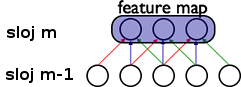
\includegraphics[width=150px]{text_images/conv_1D_nn.png}
  \caption{Zajedničke težine}
  \label{fig:conv-nn}
\end{figure}e

\end{frame}

%------------------------------------------------

\begin{frame}
\frametitle{Sloj sažimanja}

(\emph{engl.} pooling)

\begin{itemize}
  \item vrsta nelinearnog poduzorkovanja
  \item podijeli ulaznu sliku na više nepreklapajućih pravokutnika
  \item više pristupa
  \begin{itemize}
    \item sažimanje usprosječivanjem \engl{mean pooling}
    \item sažimanje maksimalnog odziva \engl{max pooling}
  \end{itemize}
  \item važnost
  \begin{itemize}
    \item smanjuje računsku složenost za gornje slojeve
    \item povećava neosjetljivost na translacije u slici
  \end{itemize}
\end{itemize}

\begin{figure}[htb]
\centering
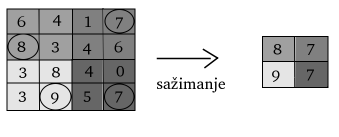
\includegraphics[scale=0.55]{text_images/max-pooling.png}
\caption{Primjer sažimanja maksimalnog odziva}
\end{figure}

\end{frame}

%------------------------------------------------
\section{Implementacija}
%------------------------------------------------

\begin{frame}
\frametitle{Theano}

\begin{itemize}
  \item alat korišten za programsku implementaciju
  \item služi za definiranje, optimiranje i prevođenje simboličkih izraza u C++ ili CUDA kod
  \item prednosti:
  \begin{itemize}
      \item autodiferenciranje - automatsko računanje gradijenata
      \item paralelno korištenje CPU i GPU (prototipiranje / evaluacija)
      \item aritmetička pojednostavljenja, na primjer: $(x \cdot y) / x \rightarrow y$
      \item ugrađene metode za poboljšanje numeričke stabilnosti određenih matematičkih izraza
  \end{itemize}
  \item mane:
  \begin{itemize}
      \item težak za učenje
      \item otklanjanje grešaka
  \end{itemize}
\end{itemize}

\end{frame}

%------------------------------------------------

\begin{frame}
\frametitle{Pretprocesiranje}

\begin{columns}[c]

\column{0.45\textwidth}
Isprobano više metoda:
  \begin{itemize}
    \item YUV kanali umjesto RGB
    \item Laplaceova piramida
    \item normalizacija vs normalizacija blokova
  \end{itemize}

\column{0.5\textwidth}
\begin{figure}[htb]
  \centering
  \includegraphics[height=0.7\textheight]{text_images/laplacian.png}
  \caption{Primjer Laplaceove piramide}
\end{figure}

\end{columns}

\end{frame}

%------------------------------------------------

\begin{frame}
\frametitle{Postprocesiranje}

\begin{itemize}
  \item koristi se metoda superpiksela - grupiranje piksela po boji ulazne slike
  \item podešavanje triju parametara
\end{itemize}

\begin{figure}[htb]
\centering
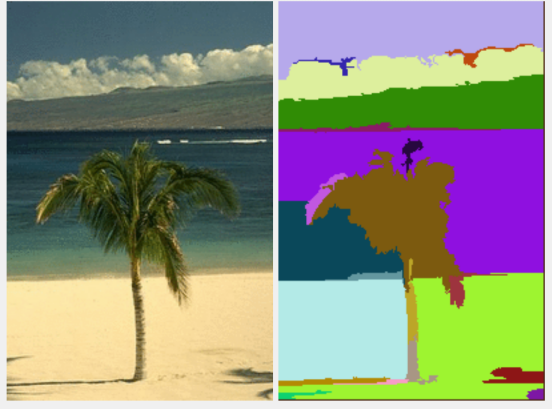
\includegraphics[scale=0.34]{text_images/superpixel.png}
\caption{Segmentacija superpikselima}
\end{figure}

\end{frame}

%------------------------------------------------

\begin{frame}
\frametitle{Arhitektura sustava}

\begin{figure}[htb]
  \centering
  \includegraphics[width=\textwidth]{text_images/arch.png}
\end{figure}

\end{frame}

%------------------------------------------------

\begin{frame}
\frametitle{Arhitektura mreže}

\begin{figure}[htb]
\centering
\includegraphics[width=\textwidth]{text_images/net.png}
\end{figure}

\begin{itemize}
  \item \textit{leakyReLU} aktivacijska fukcija
  \item 3 razine: svaka razina ima 3 sloja koja dijele filtere od 3 konvolucijska sloja
  \item na kraju je potpuno povezani sloj i sloj multinomijalne regresije koji vrši klasifikaciju određenog piksela
\end{itemize}

\end{frame}

%------------------------------------------------

\begin{frame}
\frametitle{Funkcije gubitka}

\begin{block}{Negativna log izglednost}
$ nll = - \frac{1}{N} \sum_{i=1}^{N} \ln P(Y_i = c_i)$
\end{block}

\begin{block}{Bayesova log izglednost - balansiranje razreda}
$ bayesian\_nll = - \frac{1}{N} \sum_{i=1}^{N} \frac{1}{P_{apr}(c_i)} \ln P(Y_i = c_i) $
\end{block}

$N$ je broj primjera u skupu za učenje, $P_{apr}(c_i)$ je apriorna vjerojatnost klase $c_i$, $Y_i$ je izlaz mreže.

\end{frame}

%------------------------------------------------
\section{Testni skupovi}
%------------------------------------------------

\begin{frame}
\frametitle{Stanford Background Dataset}

\begin{itemize}
  \item slike vanjskih scena, sakupljene iz raznih skupova podataka
  \item veličina 320 x 240 piksela
  \item 715 slika
  \item 8 semantičkih oznaka  % TODO navesti oznake
\end{itemize}

\begin{figure}[htb]
  \centering
  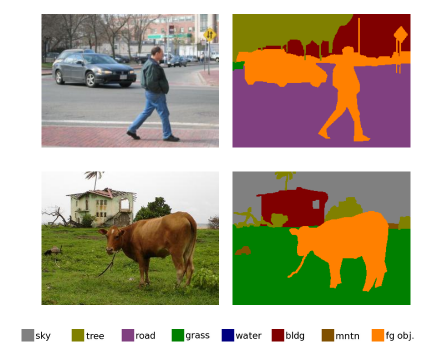
\includegraphics[scale=0.4]{text_images/dag-example.png}
  \caption{Primjer slike i oznake iz skupa Stanford Background}
\end{figure}

\end{frame}

%------------------------------------------------

\begin{frame}
\frametitle{KITTI}

\begin{itemize}
  \item slike snimljene kamerom montiranom na vozilo, veličine 1241 x 376 piksela
  \item RGB, ali i dubinska komponenta
  \item 146 označenih: 100 za učenje, 46 za testiranje
  \item 12 semantičkih oznaka  % TODO navesti oznake
\end{itemize}

\begin{figure}[htb]
  \centering
  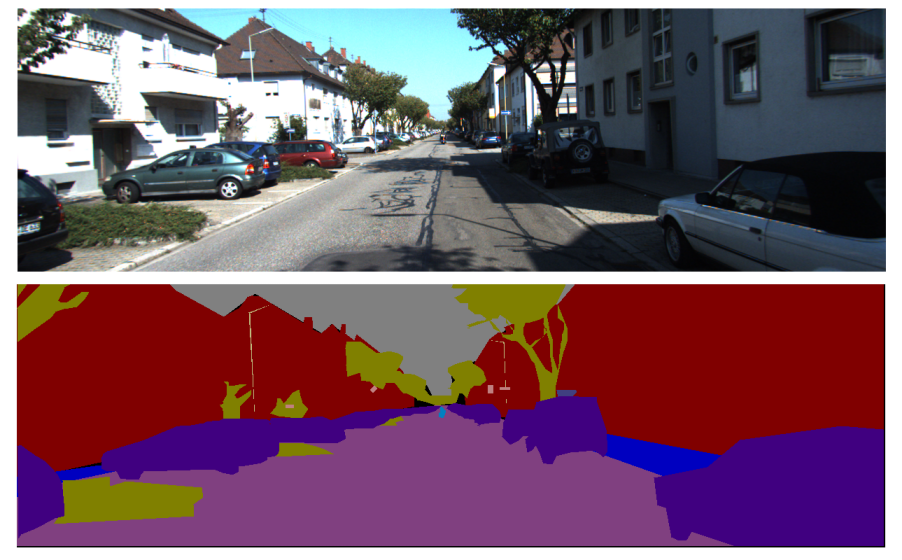
\includegraphics[scale=0.2]{text_images/kitti-example.png}
  \caption{Primjer slike i oznake iz skupa KITTI}
\end{figure}

\end{frame}

%------------------------------------------------
\section{Rezultati}
%------------------------------------------------

\begin{frame}
\frametitle{Rezultati - Stanford Background}

\begin{table}
\small
\centering

\begin{adjustbox}{center}
\begin{tabular}{l r r r}
  Metoda & Točnost(\%) & Točnost & Brzina (sec) \\
    \multicolumn{2}{c}{Funkcija troška} & razreda(\%) & \\[0.6em] \hline

  Konv. mreža s 3 razine & 75.7 & 59.3 & 0.05 \\
    \multicolumn{2}{c}{negativna log izglednost} & & \\ \hline
  Konv. mreža s 3 razine + \textit{superpixels} & 76.1 & 59.7 & 0.11 \\
    \multicolumn{2}{c}{negativna log izglednost} & & \\ \hline
  Konv. mreža s 3 razine & 71.4 & 64.8 & 0.05 \\
    \multicolumn{2}{c}{Bayesova log izglednost} & & \\ \hline
  Konv. mreža s 3 razine + \textit{superpixels} & 74.2 & 68.1 & 0.11 \\
    \multicolumn{2}{c}{Bayesova log izglednost} & & \\ \hline \hline
    
  Farabet et al. 2013 & 78.8 & 72.4 & 0.6 \\ \hline
  Farabet et al. 2013 + \textit{superpixels} & 80.4 & 74.6 & 0.7 \\ \hline
  Lempitzky et al. 2011 & 81.9 & 72.4 & >60 \\ \hline
  Munoz et al. 2010 & 76.9 & 66.2 & 12
\end{tabular}
\end{adjustbox}

\caption{Rezultati na Stanford Background skupu podataka}
\end{table}

\end{frame}

%------------------------------------------------

\begin{frame}
\frametitle{Rezultati - KITTI}

\begin{table}
\scriptsize
\centering

\begin{adjustbox}{center}
\begin{tabular}{l r r r}
  Metoda & Točnost(\%) & Točnost & Brzina (sec) \\
    \multicolumn{2}{c}{Funkcija troška} & razreda(\%) & \\[0.6em] \hline

  Konv. mreža s 3 razine (RGB) & 73.6 & 42.4 & 0.05 \\
    \multicolumn{2}{c}{negativna log izglednost} & & \\ \hline
  Konv. mreža s 3 razine (RGB) + \textit{superpixels} & 75.1 & 43.1 & 0.11 \\
    \multicolumn{2}{c}{negativna log izglednost} & & \\ \hline
  Konv. mreža s 3 razine (RGB) & 69.8 & 55.3 & 0.05 \\
    \multicolumn{2}{c}{Bayesova log izglednost} & & \\ \hline
  Konv. mreža s 3 razine (RGBD) & 78.5 & 45.8 & 0.05 \\
    \multicolumn{2}{c}{negativna log izglednost} & & \\ \hline
  Konv. mreža s 3 razine (RGBD) + \textit{superpixels} & 79.1 & 46.1 & 0.11 \\
    \multicolumn{2}{c}{negativna log izglednost} & & \\ \hline \hline
    
  Ros et al. 2015 & 81.1 & 58.0 & 0.46
\end{tabular}
\end{adjustbox}

\caption{Rezultati na KITTI skupu podataka}
\end{table}

\end{frame}

%------------------------------------------------

\begin{frame}
\frametitle{Zaključak}

U okviru ovog rada implementiran je sustav koji postiže rezultate usporedive s najboljim implementacijama. Konvolucijske neuronske mreže su se pokazale kao dobar model za semantičku segmentaciju.

\end{frame}

%------------------------------------------------

\begin{frame}
\Huge{\centerline{The End}}
\end{frame}

%------------------------------------------------

\begin{frame}
\frametitle{Neuronske mreže - uvod}

umjetni neuroni: perceptron
\begin{itemize}
  \item linearni klasifikator
  \item aktivacijska funkcija: logistički sigmoid
\end{itemize}

\begin{block}{Izlaz}
\begin{equation}
P(Y = 0 | \boldsymbol{x}, \boldsymbol{w}, b) = \sigma(\sum_{j=0}^{N} w_j \cdot x_j + b)
\label{eq:sigmoid}
\end{equation}
\end{block}
$\sigma$ -- logistička funkcija,
$\sigma(x) = \frac{1}{1 + e^{-x}}$

\begin{figure}[htb]
\centering

\includegraphics[width=120px]{text_images/percep.png}
\caption{Perceptron}
\end{figure}

\end{frame}

%------------------------------------------------

\begin{frame}
\frametitle{Neuronske mreže}

\begin{itemize}
  \item povezivanje više neurona u slojeve
  \item modeliranje kompleksnih nelinearnih zavisnosti
  \item ulazni sloj, skriveni sloj, izlazni sloj
  \item učenje algoritmom unazadne propagacije \engl{backpropagation}
  \item negativne kritike
  \begin{itemize}
    \item zapinjanje u lokalnim optimumima
    \item nestajući gradijenti \engl{vanishing gradient}
  \end{itemize}
  \item duboke mreže
  \item \textit{state-of-the-art} u većini primjera računalnog vida
\end{itemize}

\end{frame}

%------------------------------------------------

\begin{frame}
\frametitle{Konvolucijski operator}

\begin{figure}[htb]
\centering
\includegraphics[height=0.6\textheight]{text_images/kernel_convolution.jpg}
\caption{Konvolucija kroz više kanala\footnote{
https://developer.apple.com/ library/ios/documentation/Performance/Conceptual/ vImage/Art/kernel\_convolution.jpg}}
\end{figure}

\end{frame}

%------------------------------------------------
\begin{frame}
\frametitle{Prikaz konvolucije s više kanala}

\begin{figure}[htb]
\centering
\includegraphics[height=200px]{text_images/feat-maps.png}
\caption{Prikaz konvolucija}
\end{figure}

\end{frame}

%------------------------------------------------

\begin{frame}

\frametitle{Aktivacijske funkcije}

\begin{itemize}
  \item logistička sigmoid funkcija % nastavak iz neuronskih mreza
  \item hiperbolna tangens funkcija % jer joj je izlaz oko 0, pa ne unistava normalizaciju
  \item ReLU funkcije \engl{Rectified Linear Unit}
  \begin{itemize}
    \item rješava problem zasićenja gradijenata
    \item više vrsta: standardne, leaky, ...
  \end{itemize}
\end{itemize}

\begin{figure}[htb]
  \centering
  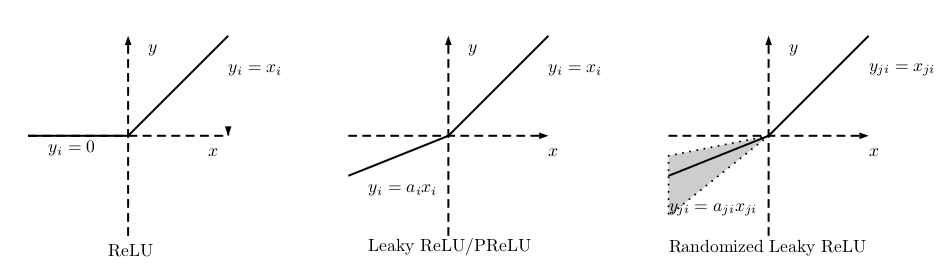
\includegraphics[scale=0.32]{text_images/relus.png}
  \caption{ReLU funkcije}
\end{figure}

\end{frame}

%------------------------------------------------

\begin{frame}
\frametitle{Regularizacija}

\begin{itemize}
  \item sprječava prenaučenost
  \item korištene tehnike
  \begin{itemize}
    \item $L_2$ regularizacija, $L_2(\boldsymbol{w}) = \norm{\boldsymbol{w}}_2 = \sum_{i = 1}^{n} {w_i}^2$
    \item umjetno povećanje skupa za učenje (slučajne transformacije)
    \begin{itemize}
      \item
        \textbf{translacije} slike po x ili y osi za neki malen pomak, na primjer 5\% slike
      \item
        \textbf{rotacije} slike za kut od $\pm 7\deg$
      \item
        \textbf{skaliranje} (uvećavanje ili smanjivanje) slike za neki faktor koji je obično u raponu od $<0.9, 1.1>$
      \item
        \textbf{smik} slike za kut od $\pm 5\deg$
    \end{itemize}
    \item \textit{dropout} - ''isključivanje'' neurona
  \end{itemize}
\end{itemize}

\end{frame}

%------------------------------------------------

\begin{frame}
\frametitle{Dropout}

\begin{figure}[htb]
\centering
\includegraphics[scale=0.55]{text_images/dropout.png}
\caption{Dropout}
\end{figure}

\end{frame}

%------------------------------------------------

\begin{frame}
\frametitle{Učenje u dva koraka}

\begin{enumerate}
  \item učenje konvolucijskih slojeva - klasifikacija pojedinog piksela samo slojem logističke (multinomijalne) regresije
  \item učenje klasifikatora - učenje potpuno povezanog sloja i sloja logističke (multinomijalne) regresije dodanih na konvolucije
\end{enumerate}

\begin{figure}[htb]
  \centering
  \includegraphics[scale=0.35]{text_images/cost-iccv1.png}
\end{figure}

\end{frame}

%------------------------------------------------

\begin{frame}[fragile]
\frametitle{Konfiguracijska programske implmentacije}

\begin{itemize}
  \item JSON format  % odabran jel se dobro preslikava u python
  \item konfiguracija parametara mreže
\end{itemize}


\begin{lstlisting}[language=json]
{
    "evaluation": {
        "batch-size": 4
    },
    "network": {
        "layers": [16, 64, 256, 1000],
        "loss": "negative_log_likelihood",
        "builder-name": "build_multiscale",
        "seed": 23451
    },
    "training": {
        "optimization": "rms",
        "optimization-params": {
            "learning-rate": 0.0002,
            "momentum": 0.9
        },
        "epochs": -1,
        "learning-rate-decrease-params": {
            "no-improvement-epochs": 4,
            "min-learning-rate": 0.00001
        }
    },
}
\end{lstlisting}

\end{frame}

%------------------------------------------------

\begin{frame}
\frametitle{Primjer mreže}

\begin{itemize}
  \item LeNet je primjer često citirane konvolucijske mreže
  \item neuron (m-1) sloja povezan samo sa prostorno bliskim neuronima m-tog sloja
  \item u početnim se slojevima izmjenjuju slojevi maksimalnog odziva i konvolucijski slojevi
  \item zadnji dio je potpuno povezani sloj na čije su ulaze spojeni izlazi zadnjeg sloja maksimalnog sažimanja
\end{itemize}

\begin{figure}
\centering
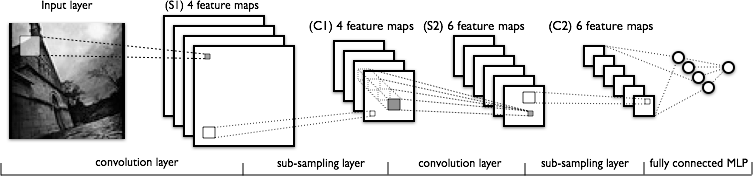
\includegraphics[width=\textwidth]{text_images/mylenet.png}
\caption{LeNet mreža}
\end{figure}

\end{frame}

%------------------------------------------------

\end{document}